\chapter{Introduction}\label{Introduction}

\paragraph{Additional reading:} Sections 2.1 (Introduction) and 2.2
(Shannon ciphers and perfect security) in the Boneh Shoup book. Chapters
1 and 2 of Katz-Lindell book.\footnote{In the current state of these
  lecture notes, almost all references and credits are omitted unless
  the name has become standard in the literature, or I believe that the
  story of some discovery can serve a pedagogical point. See the
  Katz-Lindell book for historical notes and references. This lecture
  shares a lot of text with (though is not identical to) my lecture on
  cryptography in the \href{http://introtcs.org}{introduction to
  theoretical computer science} lecture notes.}

Ever since people started to communicate, there were some messages that
they wanted kept secret. Thus cryptography has an old though arguably
\emph{undistinguished} history. For a long time cryptography shared
similar features with Alchemy as a domain in which many otherwise smart
people would be drawn into making fatal mistakes. Indeed, the history of
cryptography is littered with the figurative corpses of cryptosystems
believed secure and then broken, and sometimes with the actual corpses
of those who have mistakenly placed their faith in these cryptosystems.
The definitive text on the history of cryptography is David Kahn's ``The
Codebreakers'', whose title already hints at the ultimate fate of most
cryptosystems.\footnote{Traditionally, \emph{cryptography} was the name
  for the activity of \emph{making} codes, while \emph{cryptoanalysis}
  is the name for the activity of \emph{breaking} them, and
  \emph{cryptology} is the name for the union of the two. These days
  \emph{cryptography} is often used as the name for the broad science of
  constructing and analyzing the security of not just encryptions but
  many schemes and protocols for protecting the confidentiality and
  integrity of communication and computation.} (See also ``The Code
Book'' by Simon Singh.)

We recount below just a few stories to get a feel for this field. But
before we do so, we should introduce the \textbf{cast of characters}.
The basic setting of ``encryption'' or ``secret writing'' is the
following: one person, whom we will call \textbf{Alice}, wishes to send
another person, whom we will call \textbf{Bob}, a \textbf{secret}
message. Since Alice and Bob are not in the same room (perhaps because
Alice is imprisoned in a castle by her cousin the queen of England),
they cannot communicate directly and need to send their message in
writing. Alas, there is a third person, whom we will call \textbf{Eve},
that can see their message. Therefore Alice needs to find a way to
\emph{encode} or \emph{encrypt} the message so that only Bob (and not
Eve) will be able to understand it.

\section{Some history}\label{Some-history}

1587, Mary the queen of Scots, and the heir to the throne of England,
wanted to arrange the assassination of her cousin, queen Elisabeth I of
England, so that she could ascend to the throne and finally escape the
house arrest under which she had been for the last 18 years. As part of
this complicated plot, she sent a coded letter to Sir Anthony Babington.

\begin{marginfigure}
\centering
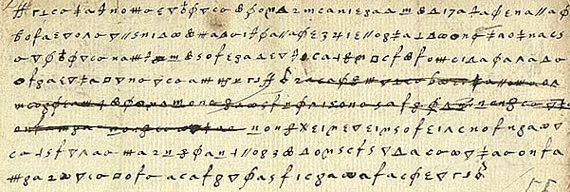
\includegraphics[width=\linewidth, height=1.5in, keepaspectratio]{../figure/encrypted_letter.jpg}
\caption{Snippet from encrypted communication between queen Mary and Sir
Babington}
\label{maryscottletterfig}
\end{marginfigure}

Mary used what's known as a \emph{substitution cipher} where each letter
is transformed into a different obscure symbol (see
\cref{maryscottletterfig}). At a first look, such a letter might seem
rather inscrutable- a meaningless sequence of strange symbols. However,
after some thought, one might recognize that these symbols \emph{repeat}
several times and moreover that different symbols repeat with different
frequencies. Now it doesn't take a large leap of faith to assume that
perhaps each symbol corresponds to a different letter and the more
frequent symbols correspond to letters that occur in the alphabet with
higher frequency. From this observation, there is a short gap to
completely breaking the cipher, which was in fact done by queen
Elisabeth's spies who used the decoded letters to learn of all the
co-conspirators and to convict queen Mary of treason, a crime for which
she was executed. Trusting in superficial security measures (such as
using ``inscrutable'' symbols) is a trap that users of cryptography have
been falling into again and again over the years. (As in many things,
this is the subject of a great XKCD cartoon, see \cref{XKCDnavajofig}.)

\begin{marginfigure}
\centering
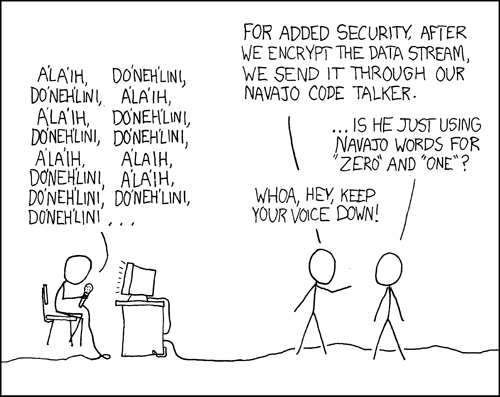
\includegraphics[width=\linewidth, height=1.5in, keepaspectratio]{../figure/code_talkers.png}
\caption{XKCD's take on the added security of using uncommon symbols}
\label{XKCDnavajofig}
\end{marginfigure}

The \href{https://en.wikipedia.org/wiki/Vigen\%C3\%A8re_cipher}{Vigenère
cipher} is named after Blaise de Vigenère who described it in a book in
1586 (though it was invented earlier by Bellaso). The idea is to use a
collection of substitution cyphers - if there are \(n\) different
ciphers then the first letter of the plaintext is encoded with the first
cipher, the second with the second cipher, the \(n^{th}\) with the
\(n^{th}\) cipher, and then the \(n+1^{st}\) letter is again encoded
with the first cipher. The key is usually a word or a phrase of \(n\)
letters, and the \(i^{th}\) substitution cipher is obtained by shifting
each letter \(k_i\) positions in the alphabet. This ``flattens'' the
frequencies and makes it much harder to do frequency analysis, which is
why this cipher was considered ``unbreakable'' for 300+ years and got
the nickname ``le chiffre indéchiffrable'' (``the unbreakable cipher'').
Nevertheless, Charles Babbage cracked the Vigenère cipher in 1854
(though he did not publish it). In 1863 Friedrich Kasiski broke the
cipher and published the result. The idea is that once you guess the
length of the cipher, you can reduce the task to breaking a simple
substitution cipher which can be done via frequency analysis (can you
see why?). Confederate generals used Vigenère regularly during the civil
war, and their messages were routinely cryptanalzed by Union officers.

\begin{marginfigure}
\centering
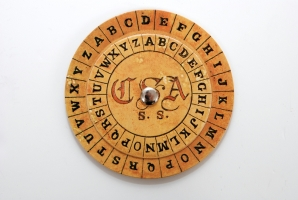
\includegraphics[width=\linewidth, height=1.5in, keepaspectratio]{../figure/confederate_cipher_disk.jpg}
\caption{Confederate Cipher Disk for implementing the Vigenère cipher}
\label{tmplabelfig}
\end{marginfigure}

\begin{marginfigure}
\centering
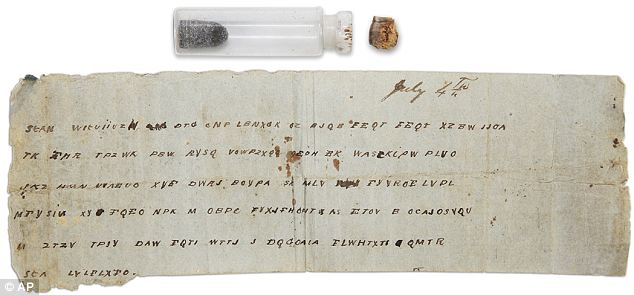
\includegraphics[width=\linewidth, height=1.5in, keepaspectratio]{../figure/confederate_message.jpg}
\caption{Confederate encryption of the message ``Gen'l Pemberton: You
can expect no help from this side of the river. Let Gen'l Johnston know,
if possible, when you can attack the same point on the enemy's lines.
Inform me also and I will endeavor to make a diversion. I have sent some
caps. I subjoin a despatch from General Johnston.''}
\label{tmplabelfig}
\end{marginfigure}

The \emph{Enigma} cipher was a mechanical cipher (looking like a
typewriter, see \cref{enigmafig}) where each letter typed would get
mapped into a different letter depending on the (rather complicated) key
and current state of the machine which had several rotors that rotated
at different paces. An identically wired machine at the other end could
be used to decrypt. Just as many ciphers in history, this has also been
believed by the Germans to be ``impossible to break'' and even quite
late in the war they refused to believe it was broken despite mounting
evidence to that effect. (In fact, some German generals refused to
believe it was broken even \emph{after} the war.) Breaking Enigma was an
heroic effort which was initiated by the Poles and then completed by the
British at Bletchley Park, with Alan Turing (of the Turing machines)
playing a key role. As part of this effort the Brits built arguably the
world's first large scale mechanical computation devices (though they
looked more similar to washing machines than to iPhones). They were also
helped along the way by some quirks and errors of the German operators.
For example, the fact that their messages ended with ``Heil Hitler''
turned out to be quite useful.

\begin{marginfigure}
\centering
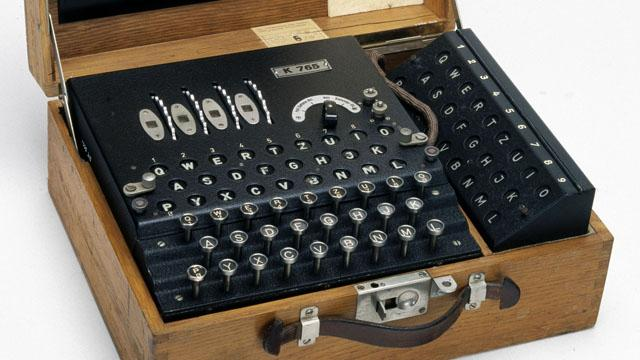
\includegraphics[width=\linewidth, height=1.5in, keepaspectratio]{../figure/enigma.jpg}
\caption{In the \emph{Enigma} mechanical cipher the secret key would be
the settings of the rotors and internal wires. As the operator types up
their message, the encrypted version appeared in the display area above,
and the internal state of the cipher was updated (and so typing the same
letter twice would generally result in two different letters output).
Decrypting follows the same process: if the sender and receiver are
using the same key then typing the ciphertext would result in the
plaintext appearing in the display.}
\label{enigmafig}
\end{marginfigure}

Here is one entertaining anecdote: the Enigma machine would never map a
letter to itself. In March 1941, Mavis Batey, a cryptanalyst at
Bletchley Park received a very long message that she tried to decrypt.
She then noticed a curious property--- the message did \emph{not}
contain the letter ``L''.\footnote{Here is a nice exercise: compute (up
  to an order of magnitude) the probability that a 50-letter long
  message composed of random letters will end up not containing the
  letter ``L''.} She realized that the probability that no ``L'''s
appeared in the message is too small for this to happen by chance. Hence
she surmised that the original message must have been composed
\emph{only} of L's. That is, it must have been the case that the
operator, perhaps to test the machine, have simply sent out a message
where he repeatedly pressed the letter ``L''. This observation helped
her decode the next message, which helped inform of a planned Italian
attack and secure a resounding British victory in what became known as
``the Battle of Cape Matapan''. Mavis also helped break another Enigma
machine. Using the information she provided, the Brits were able to feed
the Germans with the false information that the main allied invasion
would take place in Pas de Calais rather than on Normandy.

In the words of General Eisenhower, the intelligence from Bletchley park
was of ``priceless value''. It made a huge difference for the Allied war
effort, thereby shortening World War II and saving millions of lives.
See also \href{http://www.cix.co.uk/~klockstone/hinsley.htm}{this
interview with Sir Harry Hinsley}.

\section{Defining encryptions}\label{Defining-encryptions}

Many of the troubles that cryptosystem designers faced over history (and
still face!) can be attributed to not properly defining or understanding
what are the goals they want to achieve in the first place. We now turn
to actually defining what is an encryption scheme. Clearly we can encode
every message as a string of bits, i.e., an element of \(\{0,1\}^\ell\)
for some \(\ell\). Similarly, we can encode the \emph{key} as a string
of bits as well, i.e., an element of \(\{0,1\}^n\) for some \(n\). Thus,
we can think of an encryption scheme as composed of two functions. The
\emph{encryption function} \(E\) maps a secret key \(k \in \{0,1\}^n\)
and a message (known also as \emph{plaintext}) \(m\in \{0,1\}^\ell\)
into a \emph{ciphertext} \(c \in \{0,1\}^L\) for some \(L\). We write
this as \(c = E_k(m)\). The \emph{decryption function} \(D\) does the
reverse operation, mapping the secret key \(k\) and the cyphertext \(c\)
back into the plaintext message \(m\), which we write as \(m = D_k(c)\).
The basic equation is that if we use the same key for encryption and
decryption, then we should get the same message back. That is, for every
\(k \in \{0,1\}^n\) and \(m\in \{0,1\}^\ell\),

\[ m = D_k(E_k(m)) \;.\]

This motivates the following definition which attempts to capture what
it means for an encryption scheme to be \emph{valid} or ``make sense'',
regardless of whether or not it is \emph{secure}:

\hypertarget{encryptiondef}{}
\begin{definition}[Valid encryption scheme] \label[definition]{encryptiondef}

Let \(L:\N \rightarrow \N\) and \(C:\N \rightarrow \N\) be two functions
mapping natural numbers to natural numbers. A pair of polynomial-time
computable functions \((E,D)\) mapping strings to strings is a
\emph{valid private key encryption scheme} (or \emph{encryption scheme}
for short) with plaintext length function \(L(\cdot)\) and ciphertext
length function \(C(\cdot)\) if for every \(n\in \N\),
\(k\in \{0,1\}^n\) and \(x \in \{0,1\}^{L(n)}\), \(|E_k(x)|= C(n)\) and
\[
D(k,E(k,x))=x \;. \label{eqvalidenc}
\]

\end{definition}

We will often write the first input (i.e., the key) to the encryption
and decryption as a subscript and so can write \eqref{eqvalidenc} also
as \(D_k(E_k(x))=x\).

\begin{marginfigure}
\centering
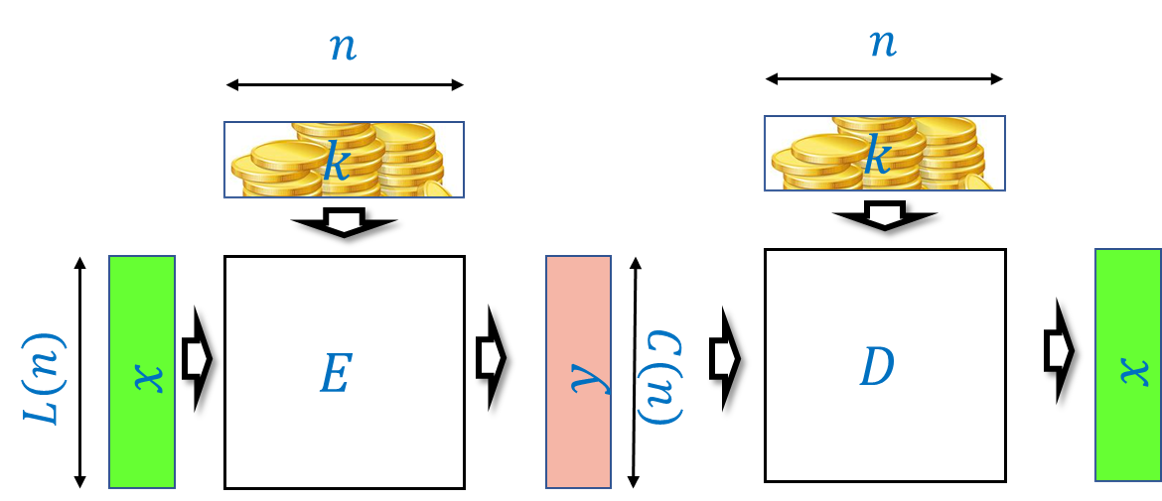
\includegraphics[width=\linewidth, height=1.5in, keepaspectratio]{../figure/encryptionvalid.png}
\caption{A private-key encryption scheme is a pair of algorithms \(E,D\)
such that for every key \(k\in \{0,1\}^n\) and plaintext
\(x\in \{0,1\}^{L(n)}\), \(y=E_k(x)\) is a ciphertext of length
\(C(n)\). The encryption scheme is \emph{valid} if for every such \(y\),
\(D_k(y)=x\). That is, the decryption of an encryption of \(x\) is
\(x\), as long as both encryption and decryption use the same key.}
\label{validencryption}
\end{marginfigure}

The validity condition implies that for any fixed \(k\), the map
\(x \mapsto E_k(x)\) is one to one (can you see why?) and hence the
ciphertext length is always at least the plaintext length. Thus we
typically focus on the plaintext length as the quantity to optimize in
an encryption scheme. The \emph{larger} \(L(n)\) is, the better the
scheme, since it means we need a shorter secret key to protect messages
of the same length.

\hypertarget{notation}{}
\begin{remark}[A note on notation, and comparison with Katz-Lindell, Boneh-Shoup, and other texts.] \label[remark]{notation}

\emph{A note on notation:} We will always use \(i,j,\ell,n\) to denote
natural numbers.

The number \(n\) will often denote the length of our secret key. The
length of the key (or another closely related number) is often known as
the \emph{security parameter} in the literature. Katz-Lindell also uses
\(n\) to denote this parameter, while Boneh-Shoup and Rosulek use
\(\lambda\) for it. (Some texts also use the greek lettter \(\kappa\)
for the same parameter.) We chose to denote the security parameter by
\(n\) as to correspond with the standard algorithmic notation for input
length (as in \(O(n)\) or \(O(n^2)\) time algorithms).

We often use \(\ell\) to denote the length of the message, sometimes
also known as ``block length'' since longer messages are simply chopped
into ``blocks'' of length \(\ell\) and also appropriately padded.

We will use \(k\) to denote the secret key, \(m\) to denote the secret
plaintext message, and \(c\) to denote the encrypted ciphertext. Note
that \(c,m\) and \(k\) are not numbers but rather bit strings of lengths
\(o,\ell\) and \(n\) respectively.

For simplicity, we denote the space of possible keys as \(\{0,1\}^n\)
and the space of possible messages as \(\{0,1\}^\ell\) for
\(\ell=L(n)\). Boneh-Shoup uses a more general notation of
\(\mathcal{K}\) for the space of all possible keys and \(\mathcal{M}\)
for the space of all possible messages. This does not make much
difference since we can represent every discrete object such as a key or
message as a binary string. (One difference is that in principle the
space of all possible messages could include messages of unbounded
length, though in such a case what is done in both theory and practice
is to break these up into finite-size blocks and encrypt one block at a
time.)

\end{remark}

\section{Defining security of
encryption}\label{Defining-security-of-encryptio}

\cref{encryptiondef} says nothing about security and does not rule out
trivial ``encryption'' schemes such as the scheme \(E_k(m) = m\) that
simply outputs the plaintext as is. Defining security is tricky, and
we'll take it one step at a time, but lets start by pondering what is
secret and what is not. A priori we are thinking of an attacker Eve that
simply sees the ciphertext \(y=E_k(x)\) and does not know anything on
how it was generated. So, it does not know the details of \(E\) and
\(D\), and certainly does not know the secret key \(k\). However, many
of the troubles past cryptosystems went through was caused by them
relying on ``security through obscurity''--- trusting that the fact
their \emph{methods} are not known to their enemy will protect them from
being broken. This is a faulty assumption - if you reuse a method again
and again (even with a different key each time) then eventually your
adversaries will figure out what you are doing. And if Alice and Bob
meet frequently in a secure location to decide on a new method, they
might as well take the opportunity to exchange their secret messages..

These considerations led Auguste Kerckhoffs in 1883 to state the
following principle:

\begin{quote}
\emph{A cryptosystem should be secure even if everything about the
system, except the key, is public knowledge.}\footnote{The actual quote
  is ``Il faut qu'il n'exige pas le secret, et qu'il puisse sans
  inconvénient tomber entre les mains de l'ennemi'' loosely translated
  as ``The system must not require secrecy and can be stolen by the
  enemy without causing trouble''. According to Steve Bellovin the NSA
  version is ``assume that the first copy of any device we make is
  shipped to the Kremlin''.}
\end{quote}

Why is it OK to assume the key is secret and not the algorithm? Because
we can always choose a fresh key. But of course that won't help us much
if our key is ``1234'' or ``passw0rd!''. In fact, if you use \emph{any}
deterministic algorithm to choose the key then eventually your adversary
will figure this out. Therefore for security we must choose the key at
\emph{random} and can restate Kerckhoffs's principle as follows:

\begin{quote}
\emph{There is no secrecy without randomness}
\end{quote}

This is such a crucial point that is worth repeating:

\begin{quote}
\emph{There is no secrecy without randomness}
\end{quote}

At the heart of every cryptographic scheme there is a secret key, and
the secret key is always chosen at random. A corollary of that is that
to understand cryptography, you need to know some probability theory.
Fortunately, we don't need much of probability- only probability over
finite spaces, and basic notions such as expectation, variance,
concentration and the union bound suffice for most of we need. In fact,
understanding the following two statements will already get you much of
what you need for cryptography:

\begin{itemize}
\item
  For every fixed string \(x\in\{0,1\}^n\), if you toss a coin \(n\)
  times, the probability that the heads/tails pattern will be exactly
  \(x\) is \(2^{-n}\).
\item
  A probability of \(2^{-128}\) is really really small.
\end{itemize}

\subsection{Generating randomness in actual cryptographic
systems}\label{Generating-randomness-in-actua}

How do we actually get random bits in actual systems? The main idea is
to use a two stage approach. First we need to get some data that is
\emph{unpredictable} from the point of view of an attacker on our
system. Some sources for this could be measuring latency on the network
or hard drives (getting harder with solid state disk), user keyboard and
mouse movement patterns (problematic when you need fresh randomness at
boot time ), clock drift and more, there are some other sources
including audio, video, and network. All of these can be problematic,
especially for servers or virtual machines, and so hardware based random
number generators based on phenomena such as thermal noise or nuclear
decay are becoming more popular. Once we have some data \(X\) that is
unpredictable, we need to estimate the \emph{entropy} in it. You can
roughly imagine that \(X\) has \(k\) bits of entropy if the probability
that an attacker can guess \(X\) is at most \(2^{-k}\). People then use
a \emph{hash function} (an object we'll talk about more later) to map
\(X\) into a string of length \(k\) which is then hopefully distributed
(close to) uniformly at random. All of this process, and especially
understanding the amount of information an attacker may have on the
entropy sources, is a bit of a dark art and indeed a number of attacks
on cryptographic systems were actually enabled by weak generation of
randomness. Here are a few examples.

One of the first attacks was on the SSL implementation of Netscape
(\emph{the} browser at the time). Netscape used the following
``unpredicatable'' information--- the time of day and a process ID both
of which turned out to be quite predictable (who knew attackers have
clocks too?). Netscape tried to protect its security through ``security
through obscurity'' by not releasing the source code for their
pseudorandom generator, but it was reverse engineered by
\href{https://www.cs.berkeley.edu/~daw/papers/ddj-netscape.html}{Ian
Goldberg and David Wagner} (Ph.D students at the time) who demonstrated
this attack.

In 2006 a programmer removed a line of code from the procedure to
generate entropy in OpenSSL package distributed by Debian since it
caused a warning in some automatic verification code. As a result for
two years (until this was discovered) all the randomness generated by
this procedure used only the process ID as an ``unpredictable'' source.
This means that all communication done by users in that period is fairly
easily breakable (and in particular, if some entities recorded that
communication they could break it also retroactively). This caused a
huge headache and a worldwide regeneration of keys, though it is
believed that many of the weak keys are still used. See
\href{http://www.xkcd.com/424/}{XKCD's take} on that incident.

\begin{figure}
\centering
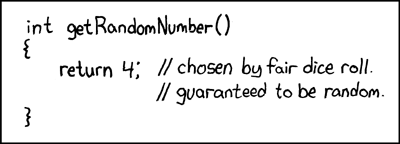
\includegraphics[width=\textwidth, height=0.25\paperheight, keepaspectratio]{../figure/random_number.png}
\caption{XKCD Cartoon: Random number generator}
\label{tmplabelfig}
\end{figure}

In 2012 two separate teams of researchers scanned a large number of RSA
keys on the web and found out that about 4 percent of them are easy to
break. The main issue were devices such as routers, internet-connected
printers and such. These devices sometimes run variants of Linux- a
desktop operating system- but without a hard drive, mouse or keyboard,
they don't have access to many of the entropy sources that desktop have.
Coupled with some good old fashioned ignorance of cryptography and
software bugs, this led to many keys that are downright trivial to
break, see
\href{https://freedom-to-tinker.com/blog/nadiah/new-research-theres-no-need-panic-over-factorable-keys-just-mind-your-ps-and-qs/}{this
blog post} and \href{https://factorable.net/}{this web page} for more
details.

After the entropy is collected and then ``purified'' or ``extracted'' to
a uniformly random string that is, say, a few hundred bits long, we
often need to ``expand'' it into a longer string that is also uniform
(or at least looks like that for all practical purposes). We will
discuss how to go about that in the next lecture. This step has its
weaknesses too and in particular the Snowden documents, combined with
observations of Shumow and Ferguson, strongly suggest that the NSA has
deliberately inserted a \emph{trapdoor} in one of the pseudorandom
generators published by the National Institute of Standards and
Technologies (NIST). Fortunately, this generator wasn't widely adapted
but apparently the NSA did pay 10 million dollars to RSA security so the
latter would make this generator their default option in their products.

\section{Defining the secrecy
requirement.}\label{Defining-the-secrecy-requireme}

Defining the secrecy requirement for an encryption is not simple. Over
the course of history, many smart people got it wrong and convinced
themselves that ciphers were impossible to break. The first person to
truly ask the question in a rigorous way was Claude Shannon in 1945
(though a partial version of his manuscript was only declassified in
1949). Simply by asking this question, he made an enormous contribution
to the science of cryptography and practical security. We now will try
to examine how one might answer it.

Let me warn you ahead of time that we are going to insist on a
\emph{mathematically precise definition} of security. That means that
the definition must capture security in all cases, and the existence of
a single counterexample, no matter how ``silly'', would make us rule out
a candidate definition. This exercise of coming up with ``silly''
counterexamples might seem, well, silly. But in fact it is this method
that has led Shannon to formulate his theory of secrecy, which (after
much followup work) eventually revolutionized cryptography, and brought
this science to a new age where Edgar Allan Poe's maxim no longer holds,
and we are able to design ciphers which human (or even nonhuman)
ingenuity cannot break.

The most natural way to attack an encryption is for Eve to guess all
possible keys. In many encryption schemes this number is enormous and
this attack is completely infeasible. For example, the theoretical
number of possibilities in the Enigma cipher was about \(10^{113}\)
which roughly means that even if we filled the milky way galaxy with
computers operating at light speed, the sun would still die out before
it finished examining all the possibilities.\footnote{There are about
  \(10^{68}\) atoms in the galaxy, so even if we assumed that each one
  of those atoms was a computer that can process say \(10^{21}\)
  decryption attempts per second (as the speed of light is \(10^9\)
  meters per second and the diameter of an atom is about \(10^{-12}\)
  meters), then it would still take \(10^{113-89} = 10^{24}\) seconds,
  which is about \(10^{17}\) years to exhaust all possibilities, while
  the sun is estimated to burn out in about 5 billion years.} One can
understand why the Germans thought it was impossible to break. (Note
that despite the number of possibilities being so enormous, such a key
can still be easily specified and shared between Alice and Bob by
writing down \(113\) digits on a piece of paper.) Ray Miller of the NSA
had calculated that, in the way the Germans used the machine, the number
of possibilities was ``only'' \(10^{23}\), but this is still extremely
difficult to pull off even today, and many orders of magnitudes above
the computational powers during the WW-II era. Thus clearly, it is
sometimes possible to break an encryption without trying all
possibilities. A corollary is that having a huge number of key
combinations does not guarantee security, as an attacker might find a
shortcut (as the allies did for Enigma) and recover the key without
trying all options.

Since it is possible to recover the key with some tiny probability
(e.g.~by guessing it at random), perhaps one way to define security of
an encryption scheme is that an attacker can never recover the key with
probability significantly higher than that. Here is an attempt at such a
definition:

\hypertarget{securefirstattemptdef}{}
\begin{definition}[Security of encryption: first attempt] \label[definition]{securefirstattemptdef}

An encyption scheme \((E,D)\) is \emph{\(n\)-secure} if no matter what
method Eve employs, the probability that she can recover the true key
\(k\) from the ciphertext \(c\) is at most \(2^{-n}\).

\end{definition}

\begin{pause} \label[pause]{When-you-see-a-mathematical-de}

When you see a mathematical definition that attempts to model some
real-life phenomenon such as security, you should pause and ask
yourself:

\begin{enumerate}
\def\labelenumi{\arabic{enumi}.}
\item
  Do I understand mathematically what is the definition stating?\\
\item
  Is it a reasonable way to capture the real life phenomenon we are
  discussing?
\end{enumerate}

One way to answer question 2 is to try to think of both examples of
objects that satisfy the definition and examples of objects that violate
it, and see if this conforms to your intuition about whether these
objects display the phenomenon we are trying to capture. Try to do this
for \cref{securefirstattemptdef}

\end{pause}

You might wonder if \cref{securefirstattemptdef} is not \emph{too
strong}. After all how are we going ever to prove that Eve cannot
recover the secret key no matter what she does? Edgar Allan Poe would
say that there can always be a method that we overlooked. However, in
fact this definition is too \emph{weak}! Consider the following
encryption: the secret key \(k\) is chosen at random in \(\{0,1\}^n\)
but our encryption scheme simply ignores it and lets \(E_k(x)=x\) and
\(D_k(y)=y\). This is a valid encryption, but of course completely
insecure as we are simply outputting the plaintext in the clear. Yet, no
matter what Eve does, if she only sees \(c\) and not \(k\), there is no
way she can guess the true value of \(k\) with probability better than
\(2^{-n}\), since it was chosen completely at random and she gets no
information about it. Formally, one can prove the following result:

\hypertarget{trivialsec}{}
\begin{lemma} \label[lemma]{trivialsec}

Let \((E,D)\) be the encryption scheme above. For every function
\(Eve:\{0,1\}^\ell\rightarrow \{0,1\}^n\) and for every
\(x\in \{0,1\}^\ell\), the probability that \(Eve(E_k(x))=k\) is exactly
\(2^{-n}\).

\end{lemma}

\begin{proof} \label[proof]{This-follows-because-Ekxx-and-}

This follows because \(E_k(x)=x\) and hence \(Eve(E_k(x))=Eve(x)\) which
is some fixed value \(k'\in\{0,1\}^n\) that is independent of \(k\).
Hence the probability that \(k=k'\) is \(2^{-n}\). QED

\end{proof}

The math behind the above argument is very simple, yet I urge you to
read and re-read the last two paragraphs until you are sure that you
completely understand why this encryption is in fact secure according to
the above definition. This is a ``toy example'' of the kind of reasoning
that we will be employing constantly throughout this course, and you
want to make sure that you follow it.

So, \cref{trivialsec} is true, but one might question its meaning.
Clearly this silly example was not what we meant when stating this
definition. However, as mentioned above, we are not willing to ignore
even silly examples and must amend the definition to rule them out. One
obvious objection is that we don't care about hiding the key- it is the
\emph{message} that we are trying to keep secret. This suggests the next
attempt:

\hypertarget{securesecondattemptdef}{}
\begin{definition}[Security of encryption: second attempt] \label[definition]{securesecondattemptdef}

An encryption scheme \((E,D)\) is \emph{\(n\)-secure} if for every
message \(x\) no matter what method Eve employs, the probability that
she can recover \(x\) from the ciphertext \(y=E_k(x)\) is at most
\(2^{-n}\).

\end{definition}

Now this seems like it captures our intended meaning. But remember that
we are being anal, and truly insist that the definition holds as stated,
namely that for every plaintext message \(x\) and every function
\(Eve:\{0,1\}^L\rightarrow\{0,1\}^\ell\), the probability over the
choice of \(k\) that \(Eve(E_k(x))=x\) is at most \(2^{-n}\). But now we
see that this is clearly impossible. After all, this is supposed to work
for \emph{every} message \(x\) and \emph{every} function \(Eve\), but
clearly if \(x\) is the all-zeroes message \(0^\ell\) and \(Eve\) is the
function that ignores its input and simply outputs \(0^\ell\), then it
will hold that \(Eve(E_k(x))=x\) with probability one.

So, if before the definition was too weak, the new definition is too
strong and is impossible to achieve. The problem is that of course we
could guess a fixed message with probability one, so perhaps we could
try to consider a definition with a \emph{random} message. That is:

\hypertarget{securethirdattemptdef}{}
\begin{definition}[Security of encryption: third attempt] \label[definition]{securethirdattemptdef}

An encyption scheme \((E,D)\) is \emph{\(n\)-secure} if no matter what
method Eve employs, if \(x\) is chosen at random from \(\{0,1\}^\ell\),
the probability that she can recover \(x\) from the ciphertext
\(c=E_k(x)\) is at most \(2^{-n}\).

\end{definition}

This weakened definition can in fact be achieved, but we have again
weakened it too much. Consider an encryption that hides the last
\(\ell/2\) bits of the message, but completely reveals the first
\(\ell/2\) bits. The probability of guessing a random message is
\(2^{-\ell/2}\), and so such a scheme would be ``\(\ell/2\) secure'' per
\cref{securethirdattemptdef} but this is still a scheme that you would
not want to use. The point is that in practice we don't encrypt random
messages--- our messages might be in English, might have common headers,
and might have even more structures based on the context. In fact, it
may be that the message is either ``Yes'' or ``No'' (or perhaps either
``Attack today'' or ``Attack tomorrow'') but we want to make sure Eve
doesn't learn which one it is. So, using an encryption scheme that
reveals the first half of the message (or frankly even only the first
bit) is unacceptable.

\section{Perfect Secrecy}\label{Perfect-Secrecy}

So far all of our attempts at definitions oscillated between being too
strong (and hence impossible) or too weak (and hence not guaranteeing
actual security). The key insight of Shannon was that in a secure
encryption scheme the ciphtertext should not reveal \emph{any additional
information} about the plaintext. So, if for example it was a priori
possible for Eve to guess the plaintext with some probability \(1/k\)
(e.g., because there were only \(k\) possibilities for it) then she
should not be able to guess it with higher probability after seeing the
ciphertext. This can be formalized as follows:

\hypertarget{perfectsecrecydef}{}
\begin{definition}[Perfect secrecy] \label[definition]{perfectsecrecydef}

An encryption scheme \((E,D)\) is \emph{perfectly secret} if there for
every set \(M\subseteq\{0,1\}^\ell\) of plaintexts, and for every
strategy used by Eve, if we choose at random \(x\in M\) and a random key
\(k\in\{0,1\}^n\), then the probability that Eve guesses \(x\) after
seeing \(E_k(x)\) is at most \(1/|M|\).

\end{definition}

In particular, if we encrypt either ``Yes'' or ``No'' with probability
\(1/2\), then Eve won't be able to guess which one it is with
probability better than half. In fact, that turns out to be the heart of
the matter:

\hypertarget{twotomanythm}{}
\begin{theorem}[Two to many theorem] \label[theorem]{twotomanythm}

An encryption scheme \((E,D)\) is perfectly secret if and only if for
every two distinct plaintexts \(\{x_0,x_1\} \subseteq \{0,1\}^\ell\) and
every strategy used by Eve, if we choose at random \(b\in\{0,1\}\) and a
random key \(k\in\{0,1\}^n\), then the probability that Eve guesses
\(x_b\) after seeing \(E_k(x_b)\) is at most \(1/2\).

\end{theorem}

\begin{proof} \label[proof]{The-only-if-direction-is-obvio}

The ``only if'' direction is obvious--- this condition is a special case
of the perfect secrecy condition for a set \(M\) of size \(2\).

The ``if'' direction is trickier. We need to show that if there is some
set \(M\) (of size possibly much larger than \(2\)) and some strategy
for Eve to guess (based on the ciphertext) a plaintext chosen from \(M\)
with probability larger than \(1/|M|\), then there is also some set
\(M'\) of size two and a strategy \(Eve'\) for Eve to guess a plaintext
chosen from \(M'\) with probability larger than \(1/2\).

Let's fix the message \(x_0\) to be the all zeroes message and pick
\(x_1\) at random in \(M\). Under our assumption, it holds that for
random key \(k\) and message \(x_1\in M\),
\[\Pr_{k \leftarrow_R \{0,1\}^n, x_1 \leftarrow_R M}[Eve(E_k(x_1))=x_1]  > 1/|M|\;.\]
On the other hand, for every choice of \(k\), \(x'= Eve(E_k(x_0))\) is a
fixed string independent on the choice of \(x_1\), and so if we pick
\(x_1\) at random in \(M\), then the probability that \(x_1=x'\) is at
most \(1/|M|\), or in other words

\[\Pr_{k \leftarrow_R \{0,1\}^n, x_1 \leftarrow_R M}[Eve(E_k(x_0))=x_1]  \leq  1/|M|\;. \label{eqhitcipher}\]

We can also write \eqref{eqhitcipher} as \[
\E_{x_1 \leftarrow_R \{0,1\}^n} \Pr[ Eve(E_k(x_0))=x_1] \leq 1/|M| 
\] and so in particular, due to linearity of expectation, there
\emph{exists} some \(x_1\) satisfying
\[ \Pr[Eve(E_k(x_1))=x_1]   > \Pr[Eve(E_k(x_0))=x_1] \;.\] (Can you see
why? This is worthwhile stopping and reading again.) But this can be
turned into an attacker \(Eve'\) such that for
\(b \leftarrow_R \{0,1\}\). the probability that \(Eve'(E_k(x_b))=x_b\)
is larger than \(1/2\). Indeed, we can define \(Eve'(y)\) to output
\(x_1\) if \(Eve(y)=x_1\) and otherwise output a random message in
\(\{ x_0 , x_1 \}\). The probability that \(Eve'(y)\) equals \(x_1\) is
higher when \(y=E_k(x_1)\) than when \(y=E_k(x_0)\), and since \(Eve'\)
outputs either \(x_0\) or \(x_1\), this means that the probability that
\(Eve'(E_k(x_b))=x_b\) is larger than \(1/2\). (Can you see why?)

\end{proof}

\begin{pause} \label[pause]{The-proof-of-creftwotomanythm-}

The proof of \cref{twotomanythm} is not trivial, and is worth reading
again and making sure you understand it. An excellent exercise, which I
urge you to pause and do now is to prove the following: \((E,D)\) is
perfectly secret if for every plaintexts \(x,x' \in \{0,1\}^\ell\), the
two random variables \(\{ E_k(x) \}\) and \(\{ E_{k'}(x') \}\) (for
randomly chosen keys \(k\) and \(k'\)) have precisely the same
distribution.

\end{pause}

\hypertarget{perfectsecrecyequiv}{}
\begin{solvedexercise}[Perfect secrecy, equivalent definition] \label[solvedexercise]{perfectsecrecyequiv}

Prove that a valid encryption scheme \((E,D)\) with plaintext length
\(L(\cdot)\) is perfectly secret if and only if for every \(n\in \N\)
and plaintexts \(x,x' \in \{0,1\}^{L(n)}\), the following two
distributions \(Y\) and \(Y'\) over \(\{0,1\}^*\) are identical:

\begin{itemize}
\item
  \(Y\) is obtained by sampling \(k\sim \{0,1\}^n\) and outputting
  \(E_k(x)\).
\item
  \(Y'\) is obtained by sampling \(k\sim \{0,1\}^n\) and outputting
  \(E_k(x')\).
\end{itemize}

\end{solvedexercise}

\begin{solution} \label[solution]{We-only-sketch-the-proof-The-c}

We only sketch the proof. The condition in the exercise is equivalent to
perfect secrecy with \(|M|=2\). For every \(M = \{ x,x' \}\), if \(Y\)
and \(Y'\) are identical then clearly for every \(Eve\),
\(\Pr[ Eve(E_k(x))=1] = \Pr[ Eve(E_k(x'))=1]\) since these correspond
applying \(Eve\) on the same distribution \(Y=Y'\). On the other hand,
if \(Y\) and \(Y'\) are not identical then there must exist some
ciphertext \(c^*\) such that \(\Pr[ Y=c^*] > \Pr[ Y'=c^*]\) (or vice
versa). The adversary that on input \(c\) will guess that \(c\) is an
encryption of \(x\) if \(c=c^*\) and otherwise will toss a coin will
have some advantage over \(1/2\) in distinguishing an encryption of
\(x\) from an encryption of \(x'\).

\end{solution}

We summarize the equivalent definitions of perfect secrecy in the
following theorem, whose (omitted) proof follows from
\cref{twotomanythm} and \cref{perfectsecrecyequiv} as well as similar
proof ideas.

\hypertarget{perfectsecrecythm}{}
\begin{theorem}[Perfect secrecy equivalent conditions] \label[theorem]{perfectsecrecythm}

Let \((E,D)\) be a valid encryption scheme with message length \(L(n)\).
Then the following conditions are equivalent:

\begin{enumerate}
\def\labelenumi{\arabic{enumi}.}
\item
  \((E,D)\) is perfectly secret as per \cref{perfectsecrecydef}.
\item
  For every pair of messages \(x_0,x_1 \in \{0,1\}^{L(n)}\), the
  distributions \(\{ E_k(x_0) \}_{k \sim \{0,1\}^n}\) and
  \(\{ E_k(x_1) \}_{k \sim \{0,1\}^n}\) are identical.
\item
  (Two-message security: Eve can't guess which of one of two messages
  was encrypted with success better than half.) For every function
  \(Eve:\{0,1\}^{C(n)} \rightarrow \{0,1\}^{L(n)}\) and pair of messages
  \(x_0,x_1 \in \{0,1\}^{L(n)}\),
\end{enumerate}

\[\Pr_{b \sim \{0,1\}, k \sim \{0,1\}^n} [ Eve(E_k(x_b))=x_b ] \leq 1/2\]

\begin{enumerate}
\def\labelenumi{\arabic{enumi}.}
\setcounter{enumi}{3}
\tightlist
\item
  (Arbitrary prior security: Eve can't guess which message was encrypted
  with success better than her prior information.) For every
  distribution \(\mathcal{D}\) over \(\{0,1\}^{L(n)}\), and
  \(Eve:\{0,1\}^{C(n)} \rightarrow \{0,1\}^{L(n)}\),
\end{enumerate}

\[\Pr_{x \sim \mathcal{D}, k \sim \{0,1\}^n}[ Eve(E_k(x))=x ] \leq max(\mathcal{D})\]

where we denote
\(max(\mathcal{D}) = \max_{x^*\in \{0,1\}^{L(n)}} \Pr_{x \sim \mathcal{D}}[x=x^*]\)
to be the largest probability of any element under \(\mathcal{D}\).

\end{theorem}

\subsection{Achieving perfect secrecy}\label{Achieving-perfect-secrecy}

So, perfect secrecy is a natural condition, and does not seem to be too
weak for applications, but can it actually be achieved? After all, the
condition that two different plaintexts are mapped to the same
distribution seems somewhat at odds with the condition that Bob would
succeed in decrypting the ciphertexts and find out if the plaintext was
in fact \(x\) or \(x'\). It turns out the answer is yes! For example,
\cref{onetimepadtwofig} details a perfectly secret encryption for two
bits.

\begin{marginfigure}
\centering
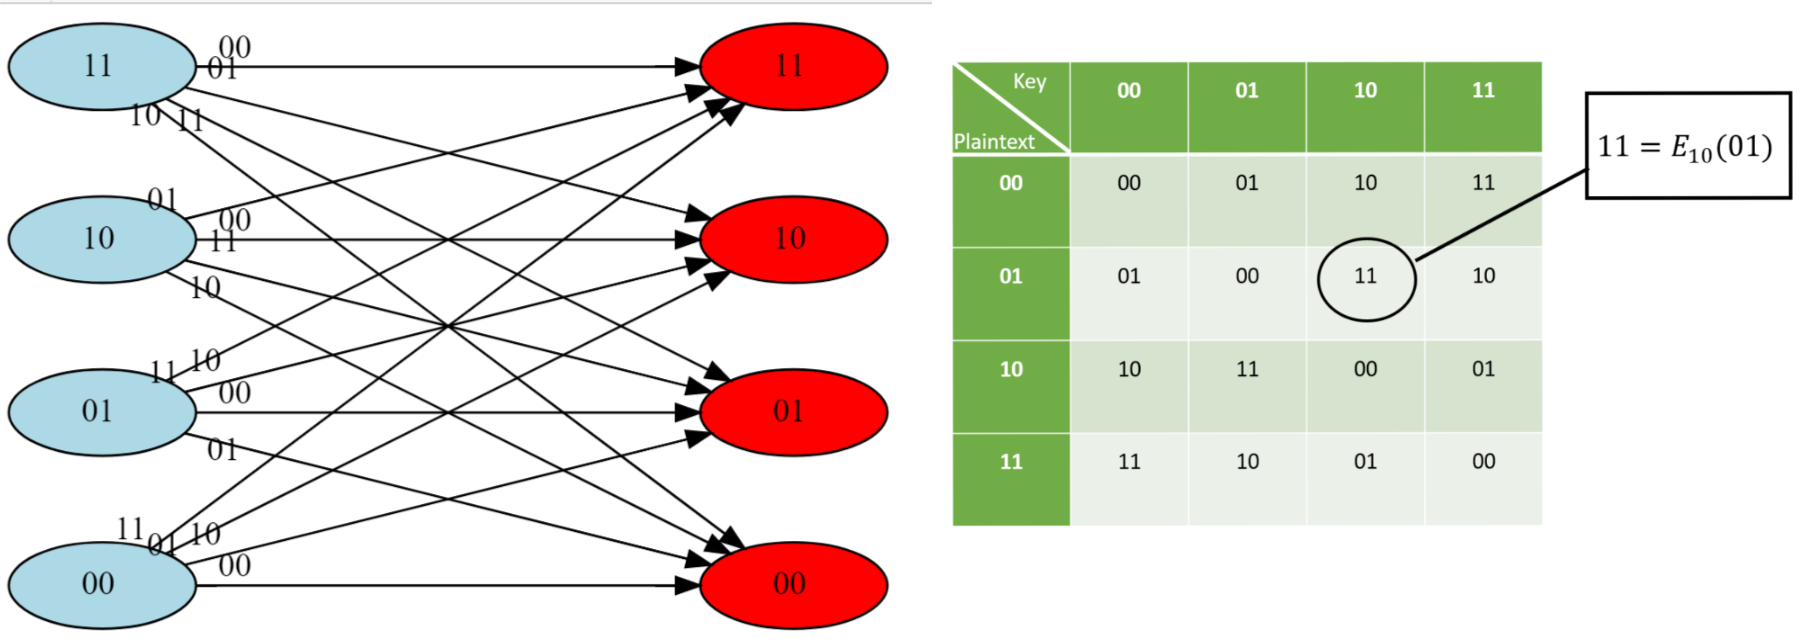
\includegraphics[width=\linewidth, height=1.5in, keepaspectratio]{../figure/onetimepadtwobits.png}
\caption{A perfectly secret encryption scheme for two-bit keys and
messages. The blue vertices represent plaintexts and the red vertices
represent ciphertexts, each edge mapping a plaintext \(x\) to a
ciphertext \(y=E_k(x)\) is labeled with the corresponding key \(k\).
Since there are four possible keys, the degree of the graph is four and
it is in fact a complete bipartite graph. The encryption scheme is valid
in the sense that for every \(k\in \{0,1\}^2\), the map
\(x \mapsto E_k(x)\) is one-to-one, which in other words means that the
set of edges labeled with \(k\) is a \emph{matching}.}
\label{onetimepadtwofig}
\end{marginfigure}

\begin{marginfigure}
\centering
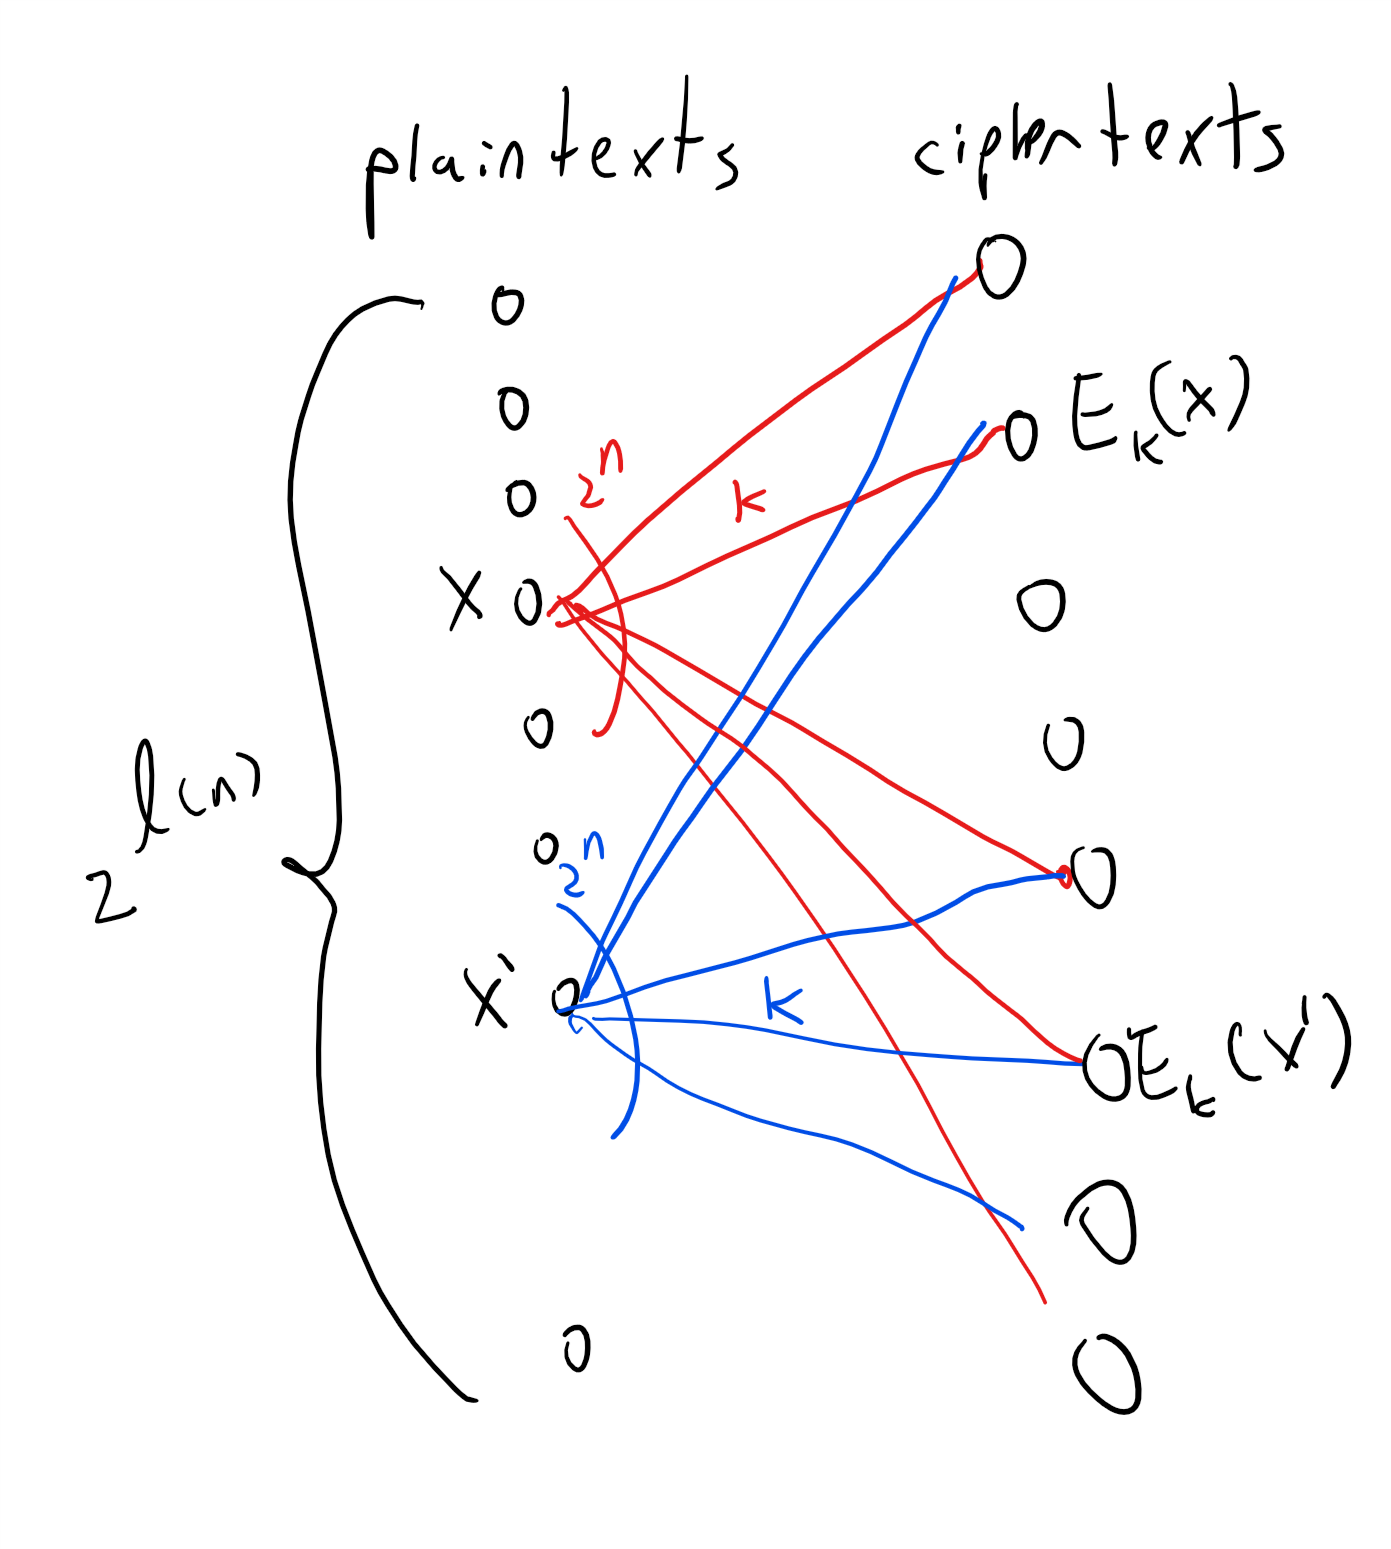
\includegraphics[width=\linewidth, height=1.5in, keepaspectratio]{../figure/perfectsecrecy.png}
\caption{For any key length \(n\), we can visualize an encryption scheme
\((E,D)\) as a graph with a vertex for every one of the \(2^{L(n)}\)
possible plaintexts and for every one of the ciphertexts in
\(\{0,1\}^*\) of the form \(E_k(x)\) for \(k\in \{0,1\}^n\) and
\(x\in \{0,1\}^{L(n)}\). For every plaintext \(x\) and key \(k\), we add
an edge labeled \(k\) between \(x\) and \(E_k(x)\). By the validity
condition, if we pick any fixed key \(k\), the map \(x \mapsto E_k(x)\)
must be one-to-one. The condition of perfect secrecy simply corresponds
to requiring that every two plaintexts \(x\) and \(x'\) have exactly the
same set of neighbors (or multi-set, if there are parallel edges).}
\label{perfectsecfig}
\end{marginfigure}

In fact, this can be generalized to any number of bits:\footnote{The
  one-time pad is typically credited to Gilbert Vernam of Bell and
  Joseph Mauborgne of the U.S. Army Signal Corps, but Steve Bellovin
  discovered an earlier inventor
  \href{http://www.cs.columbia.edu/~CS4HS/talks/FrankMillerOneTimePad.pdf}{Frank
  Miller} who published a description of the one-time pad in 1882.
  However, it is unclear if Miller realized the fact that security of
  this system can be mathematically proven, and so theorem below should
  probably be still be credited to Vernam and Mauborgne.}

\hypertarget{onetimepad}{}
\begin{theorem}[One Time Pad (Vernam 1917,  Shannon 1949)] \label[theorem]{onetimepad}

There is a perfectly secret valid encryption scheme \((E,D)\) with
\(L(n)=n\).

\end{theorem}

\begin{proofidea} \label[proofidea]{Our-scheme-is-the-one-time-pad}

Our scheme is the
\href{https://en.wikipedia.org/wiki/One-time_pad}{one-time pad} also
known as the ``Vernam Cipher'', see \cref{onetimepadfig}. The encryption
is exceedingly simple: to encrypt a message \(x\in \{0,1\}^n\) with a
key \(k \in \{0,1\}^n\) we simply output \(x \oplus k\) where \(\oplus\)
is the bitwise XOR operation that outputs the string corresponding to
XORing each coordinate of \(x\) and \(k\).

\end{proofidea}

\begin{proof}[Proof of \cref{onetimepad}] \label[proof]{For-two-binary-strings-a-and-b}

For two binary strings \(a\) and \(b\) of the same length \(n\), we
define \(a \oplus b\) to be the string \(c \in \{0,1\}^n\) such that
\(c_i = a_i + b_i \mod 2\) for every \(i\in [n]\). The encryption scheme
\((E,D)\) is defined as follows: \(E_k(x) = x\oplus k\) and
\(D_k(y)= y \oplus k\). By the associative law of addition (which works
also modulo two),
\(D_k(E_k(x))=(x\oplus k) \oplus k = x \oplus (k \oplus k) = x \oplus 0^n = x\),
using the fact that for every bit \(\sigma \in \{0,1\}\),
\(\sigma + \sigma \mod 2 = 0\) and \(\sigma + 0 = \sigma \mod 2\). Hence
\((E,D)\) form a valid encryption.

To analyze the perfect secrecy property, we claim that for every
\(x\in \{0,1\}^n\), the distribution \(Y_x=E_k(x)\) where
\(k \sim \{0,1\}^n\) is simply the uniform distribution over
\(\{0,1\}^n\), and hence in particular the distributions \(Y_{x}\) and
\(Y_{x'}\) are identical for every \(x,x' \in \{0,1\}^n\). Indeed, for
every particular \(y\in \{0,1\}^n\), the value \(y\) is output by
\(Y_x\) if and only if \(y = x \oplus k\) which holds if and only if
\(k= x \oplus y\). Since \(k\) is chosen uniformly at random in
\(\{0,1\}^n\), the probability that \(k\) happens to equal
\(x \oplus y\) is exactly \(2^{-n}\), which means that every string
\(y\) is output by \(Y_x\) with probability \(2^{-n}\).

\end{proof}

\begin{marginfigure}
\centering
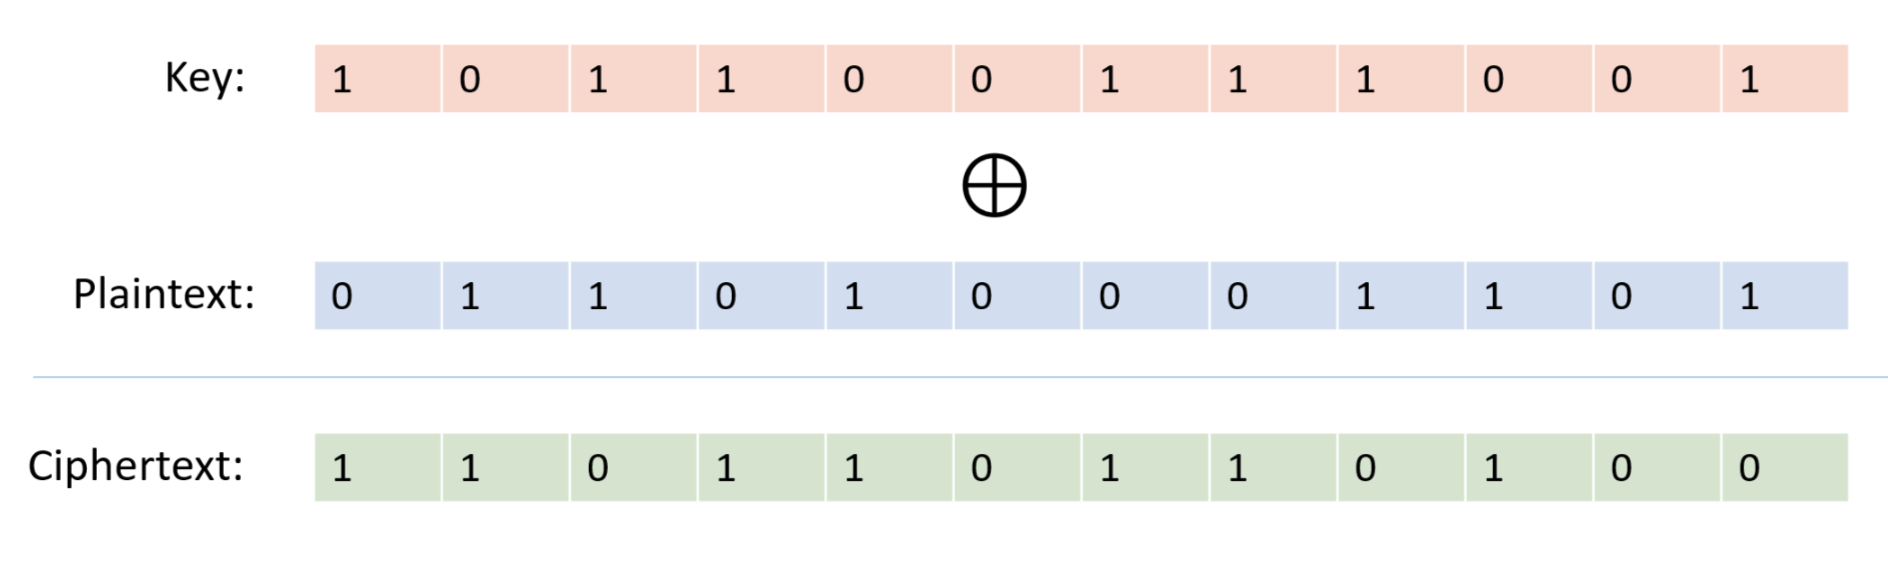
\includegraphics[width=\linewidth, height=1.5in, keepaspectratio]{../figure/onetimepad.png}
\caption{In the \emph{one time pad} encryption scheme we encrypt a
plaintext \(x\in \{0,1\}^n\) with a key \(k\in \{0,1\}^n\) by the
ciphertext \(x \oplus k\) where \(\oplus\) denotes the bitwise XOR
operation.}
\label{onetimepadfig}
\end{marginfigure}

\begin{pause} \label[pause]{The-argument-above-is-quite-si}

The argument above is quite simple but is worth reading again. To
understand why the one-time pad is perfectly secret, it is useful to
envision it as a bipartite graph as we've done in
\cref{onetimepadtwofig}. (In fact the encryption scheme of
\cref{onetimepadtwofig} is precisely the one-time pad for \(n=2\).) For
every \(n\), the one-time pad encryption scheme corresponds to a
bipartite graph with \(2^n\) vertices on the ``left side'' corresponding
to the plaintexts in \(\{0,1\}^n\) and \(2^n\) vertices on the ``right
side'' corresponding to the ciphertexts \(\{0,1\}^n\). For every
\(x\in \{0,1\}^n\) and \(k\in \{0,1\}^n\), we connect \(x\) to the
vertex \(y=E_k(x)\) with an edge that we label with \(k\). One can see
that this is the complete bipartite graph, where every vertex on the
left is connected to \emph{all} vertices on the right. In particular
this means that for every left vertex \(x\), the distribution on the
ciphertexts obtained by taking a random \(k\in \{0,1\}^n\) and going to
the neighbor of \(x\) on the edge labeled \(k\) is the uniform
distribution over \(\{0,1\}^n\). This ensures the perfect secrecy
condition.

\end{pause}

\section{Necessity of long keys}\label{Necessity-of-long-keys}

So, does \cref{onetimepad} give the final word on cryptography, and
means that we can all communicate with perfect secrecy and live happily
ever after? No it doesn't. While the one-time pad is efficient, and
gives perfect secrecy, it has one glaring disadvantage: to communicate
\(n\) bits you need to store a key of length \(n\). In contrast,
practically used cryptosystems such as AES-128 have a short key of
\(128\) bits (i.e., \(16\) bytes) that can be used to protect terabytes
or more of communication! Imagine that we all needed to use the one time
pad. If that was the case, then if you had to communicate with \(m\)
people, you would have to maintain (securely!) \(m\) huge files that are
each as long as the length of the maximum total communication you expect
with that person. Imagine that every time you opened an account with
Amazon, Google, or any other service, they would need to send you in the
mail (ideally with a secure courier) a DVD full of random numbers, and
every time you suspected a virus, you'd need to ask all these services
for a fresh DVD. This doesn't sound so appealing.

This is not just a theoretical issue. The Soviets have used the one-time
pad for their confidential communication since before the 1940's. In
fact, even before Shannon's work, the U.S. intelligence already knew in
1941 that the one-time pad is in principle ``unbreakable'' (see page 32
in the \href{http://nsarchive.gwu.edu/NSAEBB/NSAEBB278/01.PDF}{Venona
document}). However, it turned out that the hassle of manufacturing so
many keys for all the communication took its toll on the Soviets and
they ended up reusing the same keys for more than one message. They did
try to use them for completely different receivers in the (false) hope
that this wouldn't be detected. The
\href{https://en.wikipedia.org/wiki/Venona_project}{Venona Project} of
the U.S. Army was founded in February 1943 by Gene Grabeel (see
\cref{genegrabeelfig}), a former home economics teacher from Madison
Heights, Virgnia and Lt. Leonard Zubko. In October 1943, they had their
breakthrough when it was discovered that the Russians were reusing their
keys. In the 37 years of its existence, the project has resulted in a
treasure chest of intelligence, exposing hundreds of KGB agents and
Russian spies in the U.S. and other countries, including Julius
Rosenberg, Harry Gold, Klaus Fuchs, Alger Hiss, Harry Dexter White and
many others.

\begin{marginfigure}
\centering
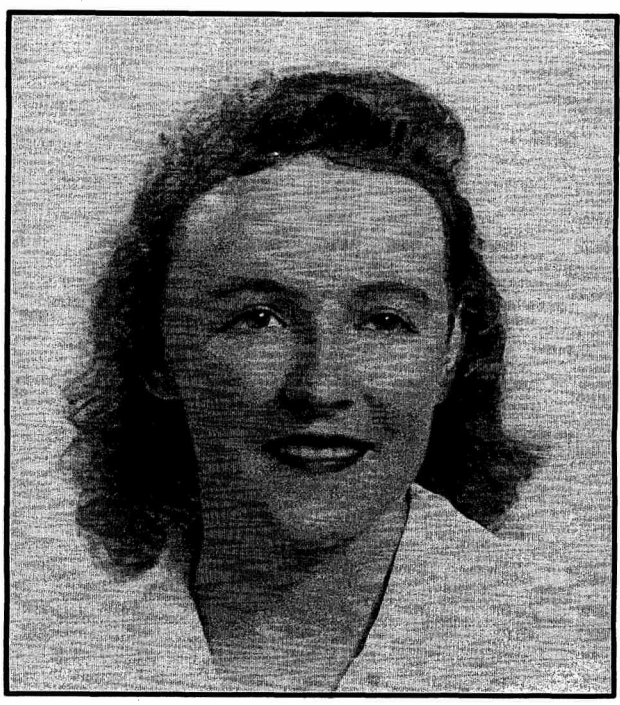
\includegraphics[width=\linewidth, height=1.5in, keepaspectratio]{../figure/genevenona.png}
\caption{Gene Grabeel, who founded the U.S. Russian SigInt program on 1
Feb 1943. Photo taken in 1942, see Page 7 in the Venona historical
study.}
\label{genegrabeelfig}
\end{marginfigure}

\begin{marginfigure}
\centering
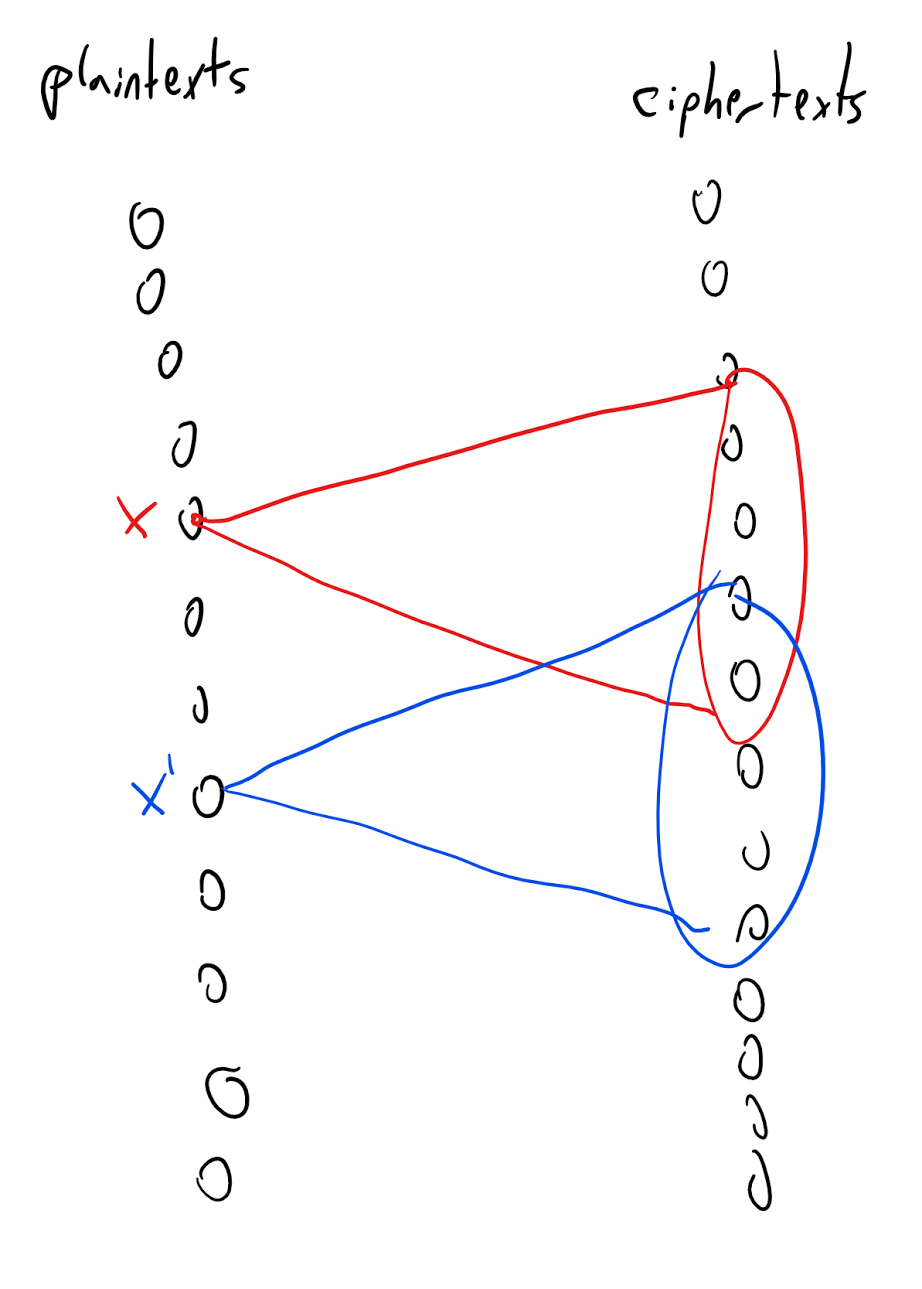
\includegraphics[width=\linewidth, height=1.5in, keepaspectratio]{../figure/longkeygraph.png}
\caption{An encryption scheme where the number of keys is smaller than
the number of plaintexts corresponds to a bipartite graph where the
degree is smaller than the number of vertices on the left side. Together
with the validity condition this implies that there will be two left
vertices \(x,x'\) with non-identical neighborhoods, and hence the scheme
does \emph{not} satisfy perfect secrecy.}
\label{longkeygraphfig}
\end{marginfigure}

Unfortunately it turns out that that such long keys are \emph{necessary}
for perfect secrecy:

\hypertarget{longkeysthm}{}
\begin{theorem}[Perfect secrecy requires long keys] \label[theorem]{longkeysthm}

For every perfectly secret encryption scheme \((E,D)\) the length
function \(L\) satisfies \(L(n) \leq n\).

\end{theorem}

\begin{proofidea} \label[proofidea]{The-idea-behind-the-proof-is-i}

The idea behind the proof is illustrated in \cref{longkeygraphfig}. We
define a graph between the plaintexts and ciphertexts, where we put an
edge between plaintext \(x\) and ciphertext \(y\) if there is some key
\(k\) such that \(y=E_k(x)\). The \emph{degree} of this graph is at most
the number of potential keys. The fact that the degree is smaller than
the number of plaintexts (and hence of ciphertexts) implies that there
would be two plaintexts \(x\) and \(x'\) with different sets of
neighbors, and hence the distribution of a ciphertext corresponding to
\(x\) (with a random key) will not be identical to the distribution of a
ciphertext corresponding to \(x'\).

\end{proofidea}

\begin{proof}[Proof of \cref{longkeysthm}] \label[proof]{Let-ED-be-a-valid-encryption-s}

Let \(E,D\) be a valid encryption scheme with messages of length \(L\)
and key of length \(n<L\). We will show that \((E,D)\) is not perfectly
secret by providing two plaintexts \(x_0,x_1 \in \{0,1\}^L\) such that
the distributions \(Y_{x_0}\) and \(Y_{x_1}\) are not identical, where
\(Y_x\) is the distribution obtained by picking \(k \sim \{0,1\}^n\) and
outputting \(E_k(x)\).

We choose \(x_0 = 0^L\). Let \(S_0 \subseteq \{0,1\}^*\) be the set of
all ciphertexts that have nonzero probability of being output in
\(Y_{x_0}\). That is,
\(S_0=\{ y \;|\; \exists_{k\in \{0,1\}^n} y=E_k(x_0) \}\). Since there
are only \(2^n\) keys, we know that \(|S_0| \leq 2^n\).

We will show the following claim:

\textbf{Claim I:} There exists some \(x_1 \in \{0,1\}^L\) and
\(k\in \{0,1\}^n\) such that \(E_k(x_1) \not\in S_0\).

Claim I implies that the string \(E_k(x_1)\) has positive probability of
being output by \(Y_{x_1}\) and zero probability of being output by
\(Y_{x_0}\) and hence in particular \(Y_{x_0}\) and \(Y_{x_1}\) are not
identical. To prove Claim I, just choose a fixed \(k\in \{0,1\}^n\). By
the validity condition, the map \(x \mapsto E_k(x)\) is a one to one map
of \(\{0,1\}^L\) to \(\{0,1\}^*\) and hence in particular the
\emph{image} of this map which is the set
\(I_k = \{ y \;|\; \exists_{x\in \{0,1\}^L} y=E_k(x) \}\) has size at
least (in fact exactly) \(2^L\). Since \(|S_0| \leq 2^n < 2^L\), this
means that \(|I_k|>|S_0|\) and so in particular there exists some string
\(y\) in \(I_k \setminus S_0\). But by the definition of \(I_k\) this
means that there is some \(x\in \{0,1\}^L\) such that
\(E_k(x) \not\in S_0\) which concludes the proof of Claim I and hence of
\cref{longkeysthm}.

\end{proof}

\hypertarget{addingprobrem}{}
\begin{remark}[Adding probability into the picture] \label[remark]{addingprobrem}

There is a sense in which both our secrecy and our impossibility results
might not be fully convincing, and that is that we did not explicitly
consider algorithms that use \emph{randomness} . For example, maybe Eve
can break a perfectly secret encryption if she is not modeled as a
deterministic function \(Eve:\{0,1\}^o\rightarrow\{0,1\}^\ell\) but
rather a \emph{probabilistic} process. Similarly, maybe the encryption
and decryption functions could be probabilistic processes as well. It
turns out that none of those matter.

For the former, note that a probabilistic process can be thought of as a
\emph{distribution} over functions, in the sense that we have a
collection of functions \(f_1,...,f_N\) mapping \(\{0,1\}^o\) to
\(\{0,1\}^\ell\), and some probabilities \(p_1,\ldots,p_N\)
(non-negative numbers summing to \(1\)), so we now think of Eve as
selecting the function \(f_i\) with probability \(p_i\). But if none of
those functions can give an advantage better than \(1/2\), then neither
can this collection (this is related to the \emph{averaging principle}
in probability).

A similar (though more involved) argument shows that the impossiblity
result showing that the key must be at least as long as the message
still holds even if the encryption and decryption algorithms are allowed
to be probabilistic processes as well (working this out is a great
exercise).

\end{remark}

\subsection{Amplifying success
probability}\label{Amplifying-success-probability}

\cref{longkeysthm} implies that for every encryption scheme \((E,D)\)
with \(L(n)>n\), there is a pair of messages \(x_0,x_1\) and an attacker
\(Eve\) that can distinguish between an encryption of \(x_0\) and an
encryption of \(x_1\) with success better than \(1/2\). But perhaps
Eve's success is only marginally better than half, say \(0.50001\)? It
turns out that's not the case. If the message is even somewhat larger
than the key, the success of Eve can be very close to \(1\):

\hypertarget{longkeyhighprob}{}
\begin{theorem}[Short keys imply high probability attack] \label[theorem]{longkeyhighprob}

Let \((E,D)\) be an encryption scheme with \(L(n)=n+t\). Then there is a
function \(Eve\) and pair of messages \(x_0,x_1\) such that
\[\Pr_{k \leftarrow_R \{0,1\}^n, b \leftarrow_R \{0,1\}}[ Eve(E_k(x_b)) = x_b] \geq 1- 2^{-t-1}\;.\]

\end{theorem}

\begin{proof} \label[proof]{As-in-the-proof-of-creflongkey}

As in the proof of \cref{longkeysthm}, let \(L=L(n)\) and let
\(x_0 = 0^L\) and \(S_0 = \{ E_k(x) : x\in \{0,1\}^n \}\) be the set of
size at most \(2^n\) of all ciphertexts corresponding to \(x_0\). We
claim that

\[\Pr_{k \leftarrow_R \{0,1\}^n , x \in \{0,1\}^\ell}[ E_k(x) \in S_0 ] \leq 2^{-t}\;. \label{eqlongkeyprobproof}\]

We show this by arguing that this bound holds for every fixed \(k\),
when we take the probability over \(x\), and so in particular it holds
also for random \(k\). Indeed, for every fixed \(k\), the map
\(x \mapsto E_k(x)\) is a one-to-one map, and so the distribution of
\(E_k(x)\) for random \(x\in \{0,1\}^n\) is uniform over some set
\(T_k\) of size \(2^{n+t}\). For every \(k\), the probability over \(x\)
that \(E_k(x) \in S_0\) is equal to
\[\tfrac{|T_k \cap S_0|}{|T_k|} \leq \tfrac{|S_0|}{|T_k|} \leq \tfrac{2^n}{2^{n+t}}=2^{-t}\]
thus proving \eqref{eqlongkeyprobproof}.

Now, for every \(x\), define \(p_x\) to be
\(\Pr_{k \leftarrow_R \{0,1\}^n}[ E_k(x) \in S_0]\). By
\eqref{eqlongkeyprobproof}, the expectation of \(p_x\) over random
\(x \leftarrow_R \{0,1\}^n\) is at most \(2^{-t}\) and so in particular
by the averaging argument \emph{there exists} some \(x_1\) such that
\(p_{x_1} \leq 2^{-t}\). Yet that means that the following adversary
\(Eve\) will be able to distinguish between an encryption of \(x_0\) and
an encryption of \(x_1\) with probability at least \(1-2^{-t-1}\):

\begin{itemize}
\item
  \textbf{Input:} A ciphertext \(y\in \{0,1\}^*\)
\item
  \textbf{Operation:} If \(y\in S_0\), output \(x_0\), otherwise output
  \(x_1\).
\end{itemize}

The probability that \(Eve(E_k(x_0))=x_0\) is equal to \(1\), while the
probability that \(Eve(E_k(x_1))=x_1\) is equal to
\(1-p_{x_1} \geq 1- 2^{-t}\). Hence the overall probability of \(Eve\)
guessing correctly is

\[
\tfrac{1}{2} \cdot 1 + \tfrac{1}{2} \cdot \left( 1-2^{-t} \right) = 1 - 2^{-t-1} \;.
\]

\end{proof}

\section{Bibliographical notes}\label{Bibliographical-notes}

Much of this text is shared with \href{https://introtcs.org}{my
Introduction to Theoretical Computer Science textbook}.

Shannon's manuscript was written in 1945 but was classified, and a
partial version was only published in 1949. Still it has revolutionized
cryptography, and is the forerunner to much of what followed.

The Venona project's history is described in
\href{http://nsarchive.gwu.edu/NSAEBB/NSAEBB278/01.PDF}{this document}.
Aside from Grabeel and Zubko, credit to the discovery that the Soviets
were reusing keys is shared by Lt. Richard Hallock, Carrie Berry, Frank
Lewis, and Lt. Karl Elmquist, and there are others that have made
important contribution to this project. See pages 27 and 28 in the
document.

In a
\href{https://www.nsa.gov/news-features/declassified-documents/nash-letters/assets/files/nash_letters1.pdf}{1955
letter to the NSA} that only recently came forward, John Nash proposed
an ``unbreakable'' encryption scheme. He wrote \emph{``I hope my
handwriting, etc. do not give the impression I am just a crank or
circle-squarer\ldots. The significance of this conjecture {[}that
certain encryption schemes are exponentially secure against key recovery
attacks{]} .. is that it is quite feasible to design ciphers that are
effectively unbreakable.''}. John Nash made seminal contributions in
mathematics and game theory, and was awarded both the Abel Prize in
mathematics and the Nobel Memorial Prize in Economic Sciences. However,
he has struggled with mental illness throughout his life. His biography,
\href{https://en.wikipedia.org/wiki/A_Beautiful_Mind_(book)}{A Beautiful
Mind} was made into a popular movie. It is natural to compare Nash's
1955 letter to the NSA to the 1956 letter by
\href{https://www.cs.cmu.edu/~aada/courses/15251s15/www/notes/godel-letter.pdf}{Kurt
Gödel to John von Neumann}. From the theoretical computer science point
of view, the crucial difference is that while Nash informally talks
about exponential vs polynomial computation time, he does not mention
the word ``Turing Machine'' or other models of computation, and it is
not clear if he is aware or not that his conjecture can be made
mathematically precise (assuming a formalization of ``sufficiently
complex types of enciphering'').
